\documentclass[colorlinks]{beamer}

\usepackage[utf8]{inputenc}
\usepackage{fancybox}
\usepackage{environ,verbatim}
\usepackage{tikz}

\newcommand{\ds}{\displaystyle}
\newcommand{\grad}{\nabla}
\newcommand{\ih}{\boldsymbol{\hat{\textbf{\i}}}}
\newcommand{\jh}{\boldsymbol{\hat{\textbf{\j}}}}
\newcommand{\vF}{\boldsymbol{\vec{\textbf{F}}}}

\beamertemplatenavigationsymbolsempty

\title{2.6 A Numerical Method (Euler's Method)}

\subtitle{a lecture for MATH F302 Differential Equations}

\author{Ed Bueler, Dept.~of Mathematics and Statistics, UAF}

\date{Fall 2023}


\usetheme{Pittsburgh}


\begin{document}

\setbeamertemplate{itemize item}{$\bullet$}
\setbeamertemplate{itemize subitem}{$\circ$}


\begin{frame}
\titlepage

\centerline{\tiny for textbook: \, D. Zill, \emph{A First Course in Differential Equations with Modeling Applications}, 11th ed.}
\end{frame}


\begin{frame}{where we stand}

\begin{itemize}
\item we now have methods for generating by-hand solutions to first-order differential equations:
    \begin{itemize}
    \item[2.2] separable equations: $y'=g(x)h(y)$
    \item[2.3] linear equations: $y'+P(x)y=f(x)$
    \item[2.4] exact equations: $M\,dx + N\,dy=0$ where $\frac{\partial M}{\partial y} = \frac{\partial N}{\partial x}$
    \end{itemize}
\item there are further methods \dots such as in section 2.5
    \begin{itemize}
    \item but \alert{we are skipping \S 2.5}; its methods are weak
    \end{itemize}

\bigskip
\item where do we stand?:
    \begin{itemize}
    \item \emph{there are some problems we can do \dots}
    \item \emph{but often our by-hand calculus/algebra techniques \alert{don't} work}
    \end{itemize}
\item this situation is permanent
\end{itemize}
\end{frame}


\begin{frame}{example 1}

\begin{itemize}
\item Example 1.  solve the initial value problem
    $$\frac{dy}{dt} = t-y^2, \qquad y(0)=1$$
in particular, find $y(4)$
\end{itemize}

\medskip
Solution version 0: \emph{Explain why 2.2--2.4 methods don't apply.}

\vspace{50mm}
\end{frame}


\begin{frame}{example 1, cont.}

Solution version 1: \emph{Solve it using a direction field and a pencil.}

\bigskip
\hfill 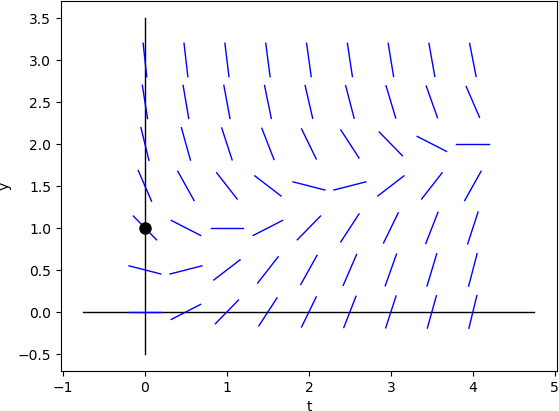
\includegraphics[width=0.7\textwidth]{figs/sequence-1}

\begin{itemize}
\item this is only approximate
\end{itemize}
\end{frame}


\begin{frame}{example 1, cont.~cont.}

Solution version 2: \emph{Make a computer follow the direction field.}

\bigskip
\hfill 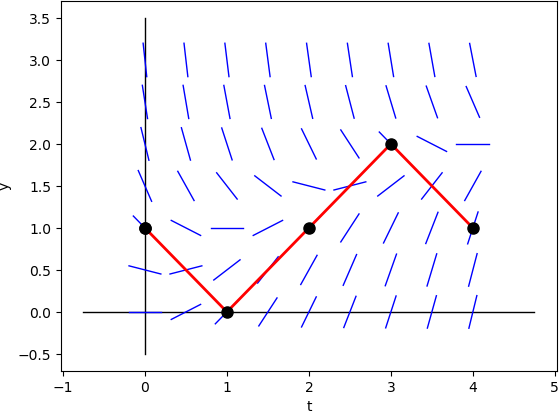
\includegraphics[width=0.7\textwidth]{figs/sequence-2}

\begin{itemize}
\item this is still only approximate because we go straight
\end{itemize}
\end{frame}


\begin{frame}{example 1, cont.~cont.~cont.}

Solution version 3: \emph{The direction field is not actually needed.}

\bigskip
\hfill 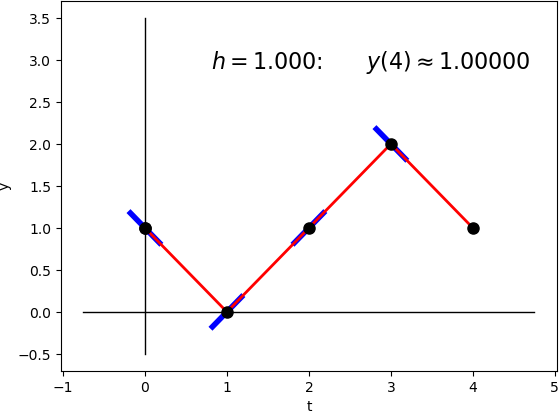
\includegraphics[width=0.7\textwidth]{figs/sequence-3}

\begin{itemize}
\item this is the same as previous
\end{itemize}
\end{frame}


\begin{frame}{example 1, cont.~cont.~cont.~cont.}

Solution version 4: \emph{Do it more accurately by smaller steps}

\bigskip
\hfill 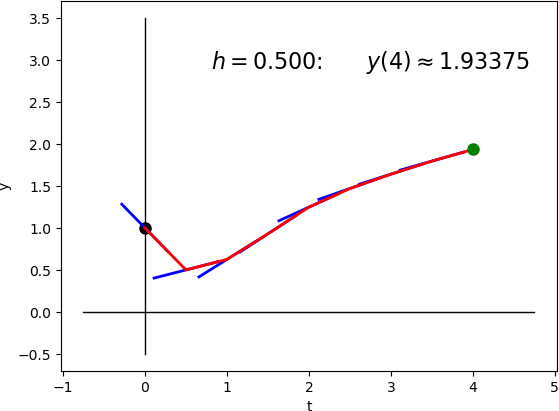
\includegraphics[width=0.7\textwidth]{figs/sequence-4}

\begin{itemize}
\item the blue slope lines are not really needed \dots
\end{itemize}
\end{frame}


\begin{frame}{example 1, cont.$^5$}

Solution version 5: \emph{Smaller steps.}

\bigskip
\hfill 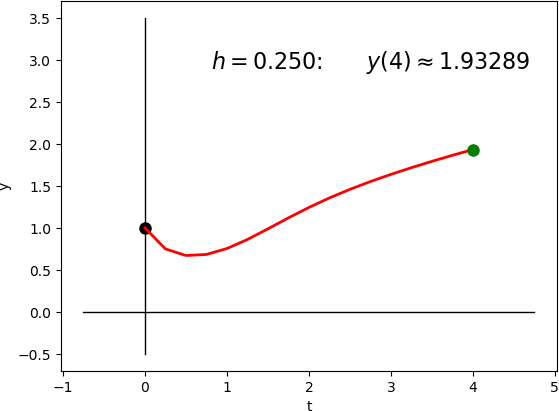
\includegraphics[width=0.7\textwidth]{figs/sequence-5}

\begin{itemize}
\item this is \emph{still} only approximate
\end{itemize}
\end{frame}


\begin{frame}{example 1, cont.$^6$}

Solution version 6: \emph{Smaller.  (Make the computer do more work.)}

\bigskip
\hfill 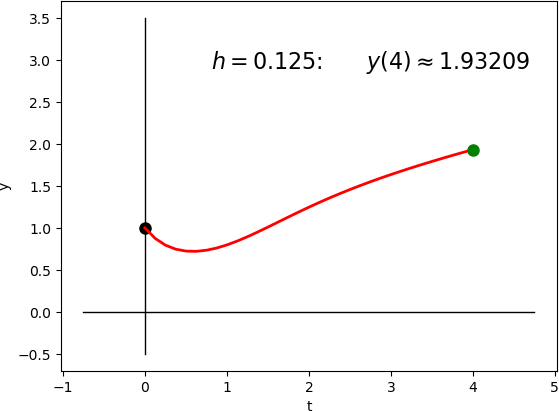
\includegraphics[width=0.7\textwidth]{figs/sequence-6}

\begin{itemize}
\item this looks like a \emph{solution} not a direction field 
\end{itemize}
\end{frame}


\begin{frame}{Euler's method}

\begin{itemize}
\item the idea of following the direction field, in a straight line for a short distance, and repeating, is \emph{Euler's method}
\item for the general DE $\frac{dy}{dx} = f(x,y)$, Euler's method is
\begin{equation}
    y_{n+1} = y_n + h\, f(x_n,y_n)   \tag{$\ast$}
\end{equation}

\vspace{-2mm}
    \begin{itemize}
    \item $h\ne 0$ is a step size \emph{you must choose}
    \item the next $x$-value is always $h$ away from the last: $x_{n+1} = x_n + h$
    \item ($\ast$) is a formula to understand \emph{and} memorize
    \item \dots and put in computer programs
    \end{itemize}
\item in the previous slides we had $f(x,y)=x-y^2$, starting values $(x_0,y_0)=(0,1)$, and four values of $h$: $h=1,0.5,0.25,0.125$
\end{itemize}
\end{frame}


\begin{frame}{a derivation of Euler's method}

easy to derive it from the direction field of $\frac{dy}{dx} = f(x,y)$, as follows:
\begin{itemize}
\item suppose we are at a point $(x_n,y_n)$
    \begin{itemize}
    \item this might be the initial point $(x_0,y_0)$
    \end{itemize}
\item the slope is $m=f(x_n,y_n)$ so the line we want is
    $$y-y_n = f(x_n,y_n)(x-x_n)$$
\item we want to move to a new location $x_{n+1}=x_n+h$ so $x-x_n=h$ and $y=y_{n+1}$
\item thus
    $$y_{n+1} - y_n = f(x_n,y_n)\, h$$
\item i.e.~$y_{n+1} = y_n + h\, f(x_n,y_n)$
\end{itemize}
\end{frame}


\begin{frame}{measuring accuracy}

\begin{itemize}
\item assume we are solving an ODE IVP:  \, $\frac{dy}{dx} = f(x,y)$, $y(x_0)=y_0$
\item if we \alert{also know the exact solution $y(x)$} then we can measure (evaluate) the error in the approximation
    $$y_n \approx y(x_n)$$
    \vspace{-4mm}
    \begin{itemize}
    \item ``$y_n$'' is the number produced by Euler's method
    \item ``$y(x_n)$'' is the exact solution at the $x$-value $x_n$
    \end{itemize}
\item picture this:
\end{itemize}

\vspace{25mm}
\end{frame}


\begin{frame}{measuring accuracy}

\begin{itemize}
\item context:
\begin{align*}
\frac{dy}{dx} &= f(x,y), \qquad y(x_0)=y_0 \\
y(x) &= (\text{exact solution, a formula}) \\
y_n &= (\text{numbers you compute from Euler's method})
\end{align*}
\item there are two common ways to report the error:
    \begin{enumerate}
    \medskip
    \item \emph{absolute error} $=|y(x_n) - y_n|$
    
    \medskip
    \item \emph{relative error} $\ds=\frac{|y(x_n) - y_n|}{|y(x_n)|}$
    \end{enumerate}
\end{itemize}
\end{frame}


\begin{frame}{caveat about measuring accuracy}

\begin{itemize}
\item you can only compute absolute or relative error \emph{if} the exact solution is known
\item \dots but usually the reason we use a numerical method like Euler's is because the exact solution is \emph{not} known
    \begin{itemize}
    \item[$\circ$] in real applications we do not know the exact solution
    \end{itemize}
\item thus: \alert{examples where the absolute or relative error is computable are automatically ``toy examples''}
\end{itemize}
\end{frame}


\begin{frame}{example 2}

\begin{itemize}
\item Example 2:  for the ODE IVP
    $$y'=y, \quad y(0)=1$$

    \begin{itemize}
    \item[(a)] find the exact solution
    \item[(b)] use Euler's method to get an approximation of $y(1)$ which is accurate to four digits?
        \begin{itemize}
        \item[$\circ$] try $h=0.1$ first, and then $h=0.05$?
        \end{itemize}
    \item[(c)] show in a table: $x_n$, $y_n$, the exact value $y(x_n)$, the absolute error, and the relative error
    \end{itemize}
\end{itemize}

\vspace{40mm}
\end{frame}


\begin{frame}[fragile]
\frametitle{example 2, cont.}

\begin{itemize}
\item so one can proceed by hand, but its tedious work \dots
\item \alert{this is the original purpose for which computers were designed}
\item I used Matlab code below
    \begin{itemize}
    \item posted as \texttt{simpleeuler.m} at the Codes tab on the public site
    \end{itemize}
\end{itemize}

\medskip
{\footnotesize
\begin{Verbatim}
h = 0.1;               % change to e.g. h=0.05
N = 10;                % change to e.g. N=20
x = 0;
y = 1;
for n = 1:N+1
    exact = exp(x);
    [x, y, exact, abs(y-exact), 100*abs(y-exact)/abs(exact)]
    y = y + h * y;     % this is Euler's method
    x = x + h;
end
\end{Verbatim}
}
\end{frame}


\begin{frame}{example 2, cont.~cont.}

\begin{itemize}
\item the code produces the table below when $h=0.1$ and we take $N=10$ steps \dots giving $4.58\%$ relative error at $x=1$

\medskip
\footnotesize
\begin{tabular}{ccccc}
$x_n$ & $y_n$ & actual value & abs.~error & rel.~error \\ \hline
0.00 & 1.0000 & 1.0000 & 0.0000 & 0.00 \\
0.10 & 1.1000 & 1.1052 & 0.0052 & 0.47 \\
0.20 & 1.2100 & 1.2214 & 0.0114 & 0.93 \\
0.30 & 1.3310 & 1.3499 & 0.0189 & 1.40 \\
0.40 & 1.4641 & 1.4918 & 0.0277 & 1.86 \\
0.50 & 1.6105 & 1.6487 & 0.0382 & 2.32 \\
0.60 & 1.7716 & 1.8221 & 0.0506 & 2.77 \\
0.70 & 1.9487 & 2.0138 & 0.0650 & 3.23 \\
0.80 & 2.1436 & 2.2255 & 0.0820 & 3.68 \\
0.90 & 2.3579 & 2.4596 & 0.1017 & 4.13 \\
1.00 & 2.5937 & 2.7183 & 0.1245 & 4.58
\end{tabular}
\end{itemize}
\end{frame}


\begin{frame}{example 2, cont.$^3$; $h=0.05$, $N=20$ case}

\scriptsize
\begin{tabular}{ccccc}
$x_n$ & $y_n$ & actual value & abs.~error & rel.~error \\ \hline
0.00 & 1.0000 & 1.0000 & 0.0000 & 0.00 \\
0.05 & 1.0500 & 1.0513 & 0.0013 & 0.12 \\
0.10 & 1.1025 & 1.1052 & 0.0027 & 0.24 \\
0.15 & 1.1576 & 1.1618 & 0.0042 & 0.36 \\
0.20 & 1.2155 & 1.2214 & 0.0059 & 0.48 \\
0.25 & 1.2763 & 1.2840 & 0.0077 & 0.60 \\
0.30 & 1.3401 & 1.3499 & 0.0098 & 0.72 \\
0.35 & 1.4071 & 1.4191 & 0.0120 & 0.84 \\
0.40 & 1.4775 & 1.4918 & 0.0144 & 0.96 \\
0.45 & 1.5513 & 1.5683 & 0.0170 & 1.08 \\
0.50 & 1.6289 & 1.6487 & 0.0198 & 1.20 \\
0.55 & 1.7103 & 1.7333 & 0.0229 & 1.32 \\
0.60 & 1.7959 & 1.8221 & 0.0263 & 1.44 \\
0.65 & 1.8856 & 1.9155 & 0.0299 & 1.56 \\
0.70 & 1.9799 & 2.0138 & 0.0338 & 1.68 \\
0.75 & 2.0789 & 2.1170 & 0.0381 & 1.80 \\
0.80 & 2.1829 & 2.2255 & 0.0427 & 1.92 \\
0.85 & 2.2920 & 2.3396 & 0.0476 & 2.04 \\
0.90 & 2.4066 & 2.4596 & 0.0530 & 2.15 \\
0.95 & 2.5270 & 2.5857 & 0.0588 & 2.27 \\
1.00 & 2.6533 & 2.7183 & 0.0650 & 2.39
\end{tabular}
\end{frame}


\begin{frame}{example 2, cont.$^4$}

\begin{center}
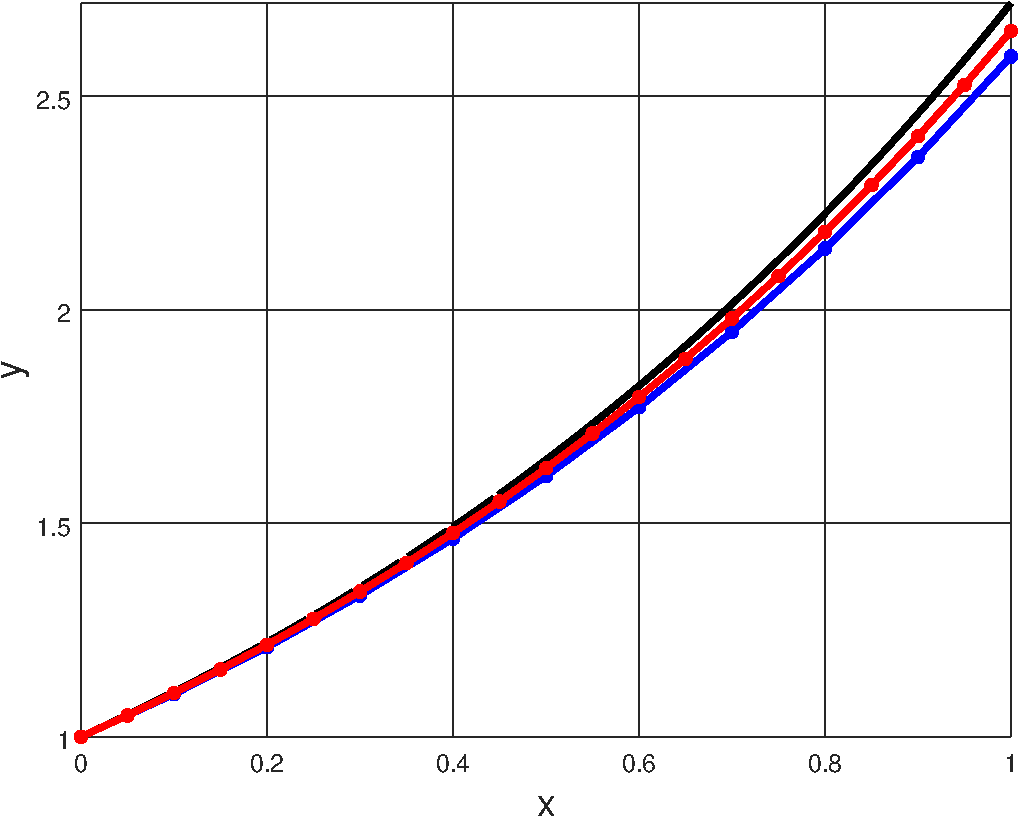
\includegraphics[width=0.8\textwidth]{figs/simpleeuler}
\end{center}

\footnotesize
\begin{itemize}
\item for $h=0.001$ and $N=1000$ I get 0.05\% rel.~error:
   $$y_{1000} = 2.71692 \approx 2.71828 = y(1)$$
\end{itemize}
\end{frame}


\begin{frame}{another derivation of Euler's method}

\begin{itemize}
\item start with the DE
    $$\frac{dy}{dx} = f(x,y)$$
\item remember what a derivative is!:
    $$\lim_{h\to 0} \frac{y(x+h)-y(x)}{h} = f(x,y(x))$$
\item think: $y(x)$ is current value and $y(x+h)$ is next value
\item drop the limit and adopt this as a method:
    $$\frac{y_{n+1}-y_n}{h} = f(x_n,y_n)$$

\vspace{-2mm}
    \begin{itemize}
    \item at this point $y_n$ and $y(x_n)$ mean different things!
    \end{itemize}
\item rewrite as Euler's method before:  $y_{n+1} = y_n + h f(x_n,y_n)$
\end{itemize}
\end{frame}


\begin{frame}{are there better methods?}

\begin{itemize}
\item yes!
\item here is a derivation, by picture, of the ``explicit midpoint rule'':
\end{itemize}

\vspace{60mm}
\end{frame}


\begin{frame}{are there better methods?}

\begin{itemize}
\item yes!
\item Euler's method is only first order; it makes errors proportional to the step size $h$
\item see the \href{https://en.wikipedia.org/wiki/Midpoint_method}{Wikipedia page for ``midpoint method''}
    \begin{itemize}
    \item[$\circ$] the explicit and implicit midpoint methods are ``second order''
    \item[$\circ$] they can get the same accuracy in 10 steps that Euler does in 100 steps
    \end{itemize}
\item see the \href{https://en.wikipedia.org/wiki/Runge-Kutta_methods}{Wikipedia page for ``Runge-Kutta methods''}
    \begin{itemize}
    \item[$\circ$] the original RK method is ``fourth order'' so it can get the same accuracy in 10 steps that Euler does in 10000 steps
    \item[$\circ$] we will return to this in Chapter 9
    \end{itemize}
\end{itemize}
\end{frame}


\begin{frame}{example 3}

\begin{itemize}
\item Example 3:  consider the ODE IVP
    $$\frac{dT}{dt} = - 0.3 \left(T - T_m(t)\right), \quad T(0)=140$$
where \quad $\ds T_m(t) = 75 - \left(\frac{60}{\pi}\right) \left(\frac{\pi}{2} + \arctan(10 (t - 5))\right)$
\item what situation does this model?
\end{itemize}

\centering
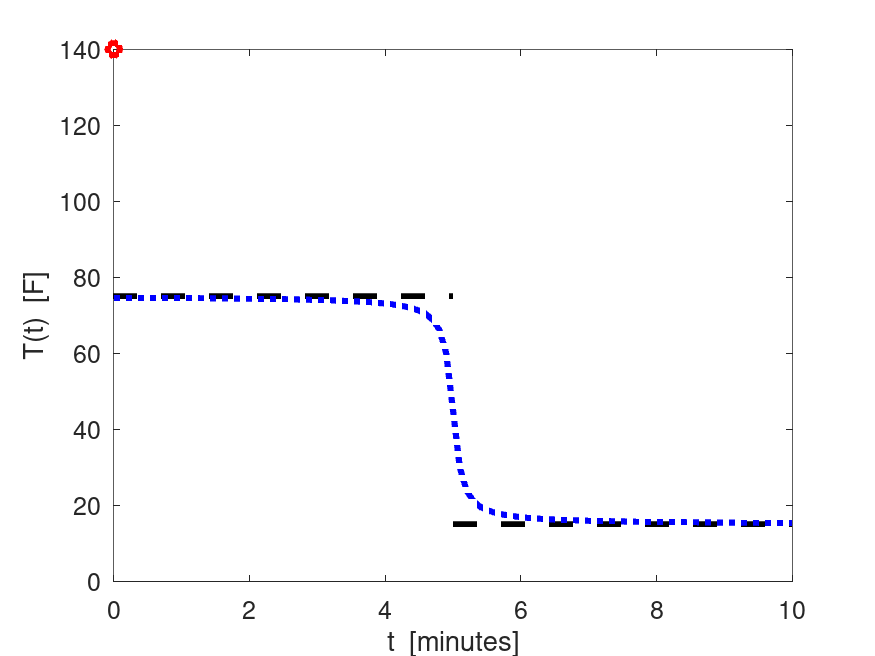
\includegraphics[width=0.6\textwidth]{figs/beforewalk.png}
\end{frame}


\begin{frame}{example 3: Newton's law of cooling}

\begin{itemize}
\small
\item consider: ODE IVP $\ds\frac{dT}{dt} = - 0.3 \left(T - T_m(t)\right)$, $T(0)=140$, where $\ds T_m(t)$ is a step down from 75 to 15 at $t=5$

\normalsize
%Use the Euler method to solve a Newton's
% law of cooling model for a cup of coffee.  You
% carry it from a warm room to the cold outside:
%    T'(t) = - 0.3 (T(t) - T_m(t))
%    T(0) = 140
% where
%    T_m(t) = 75 - (60/pi) (pi/2 + arctan(10 (t - 5)))
% This plots T(t) in red and T_m(t) in blue on
% 0 <= t <= 10.  Units: t minutes, T(t) Fahrenheit.
    
\item approximate solution using Euler's method on $t\in[0,10]$:
	$$T_{n+1} = T_n + h \left[- 0.3 \left(T - T_m(t_n)\right)\right]$$
\item try $N=50$ steps of length $\ds h=10/50 = 0.2$ minutes?
\end{itemize}

\centering
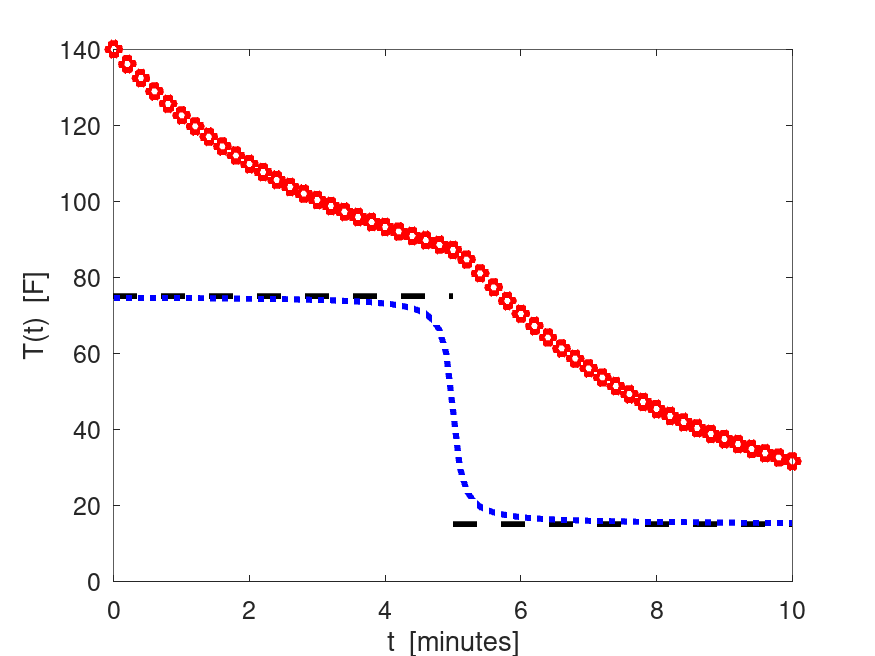
\includegraphics[width=0.6\textwidth]{figs/walkoutside.png}
\end{frame}


\begin{frame}{expectations}

\begin{itemize}
\item to learn this material, just listening to a lecture is \emph{not} enough!

\item also:
     \begin{itemize}
     \item \emph{read} section 2.6 in the textbook
     \item \emph{try out} the Euler's method codes at the \href{https://bueler.github.io/math302/codes.html}{Codes tab}
     \item \emph{do} Homework 2.6
     \end{itemize}
\end{itemize}
\end{frame}


\end{document}

